\documentclass[12pt,letterpaper]{beamer}
\usepackage[utf8]{inputenc}
\usepackage{amsmath}
\usepackage{amsfonts}
\usepackage{amssymb}
\usepackage{graphicx}
\usepackage{setspace}
\usepackage{color}
\usepackage{listings}
\usepackage{textcomp}
\usepackage{tikz}
\usetikzlibrary{automata,positioning}

\lstset{
  language=Scheme
}
\usetheme{CambridgeUS}

\title{Fizz and Fuse Your Arrays}
\author{Mike Vollmer}
\institute{Indiana University}
\date{PL Wonks, 23 October 2015}

\begin{document}

\frame{\titlepage}

\begin{frame}
  \frametitle{Fission and Fusion}
  \begin{itemize}
  \item \textbf{Fusion} combines operations on arrays.
  \item \textbf{Fission} splits up operations on arrays.
  \end{itemize}
\end{frame}

\section{Fusion}

\begin{frame}
\frametitle{What is Fusion?}
\begin{columns}[c]
\begin{column}[c]{5cm}
Functional programs often allocate lots of intermediary data structures.\\
\textbf{Fusion} is an optimization that addresses this problem.
\end{column}
\begin{column}[c]{5cm}
\begin{figure}
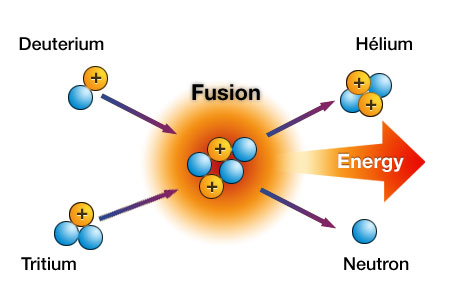
\includegraphics[width=4cm]{whatisfusion.jpg}
\end{figure}
\end{column}
\end{columns}
\end{frame}

\begin{frame}[fragile]
\frametitle{Removing Intermediary Structures}
For example, these two {\tt map} calls:
\begin{lstlisting}
(map f (map g ls))
\end{lstlisting}
The inner {\tt (map g ls)} is executed first, and it
allocates a list of {\tt g} applied to every element of
{\tt ls}. \\
If we compose {\tt f} and {\tt g}, we get:
\begin{lstlisting}
(let ([f (lambda (x) (f (g x)))])
  (map f ls))
\end{lstlisting}
\end{frame}


\section{Programming with Arrays}

\begin{frame}[fragile]
\frametitle{An Array at a Time}
Programming with arrays is convenient.
\begin{lstlisting}
(define scalar-product
  (lambda (a b)
    (vector-sum (vector-map * a b))))
\end{lstlisting}
But it can be troublesome. What is the problem with this
function?
\end{frame}

\section{Pull Arrays}

\begin{frame}[fragile]
\frametitle{Pull Arrays}
What if we \textbf{change the representation} of our arrays? \\
Instead of representing arrays directly as Scheme vectors, we can use a function from indices to values.
\begin{lstlisting}
(define pull
  (lambda (f len) 
    `(pull ,f ,len)))
\end{lstlisting}
  \begin{itemize}
  \item Each element of an array is computed independently, allowing for easy
    parallelization.
  \item The consumer of a {\tt pull array} can decide how to schedule the computations.
  \end{itemize}
\end{frame}

\begin{frame}[fragile]
\frametitle{Pull Arrays}
Converting pull arrays to scheme vectors is easy, using {\tt build-vector}. 
\begin{lstlisting}
(define pull->vector
  (lambda (arr)
    (match arr
      [`(pull ,f ,len)
       (build-vector len f)])))
\end{lstlisting}
We can also go the other way:
\begin{lstlisting}
(define vector->pull
  (lambda (vect) 
    (let ([f (lambda (i) (vector-ref vect i))]
          [len (vector-length vect)])
      (pull f len))))
\end{lstlisting}
\end{frame}

\begin{frame}[fragile]
\frametitle{Pull Arrays}
Now, {\tt map} is very simple! Maybe.
\begin{lstlisting}
(define map
  (lambda (f arr) 
    (match arr
      [`(pull ,g ,len)
       (let ([h (lambda (i) (f (g i)))])
         (pull h len))])))
\end{lstlisting}
And it looks more than a bit like our early example of fusion.
\end{frame}

\begin{frame}[fragile]
\frametitle{Pull Arrays}
Like {\tt map}, but with two array arguments.
\begin{lstlisting}
(define zipwith
  (lambda (f arr1 arr2)
    (match-let
        ([`(pull ,f1 ,len1) arr1]
         [`(pull ,f2 ,len2) arr2])
      (let ([g (lambda (i) (f (f1 i) (f2 i)))]
            [len (min len1 len2)])
        (pull g len)))))
\end{lstlisting}
The resulting array length is the minimum of the two
input lengths.
\end{frame}

\begin{frame}[fragile]
\frametitle{Pull Arrays}
To fold/reduce an array, we just loop over the length of the array.
\begin{lstlisting}
(define fold
  (lambda (f init arr)
    (match arr
      [`(pull ,g ,len)
        (let loop ([acc init] [i 0])
          (if (= i len) acc
              (loop (f acc (g i)) (add1 i))))])))
\end{lstlisting}
\end{frame}

\begin{frame}[fragile]
\frametitle{Scalar Product}
\begin{lstlisting}
(let ([a (pull f1 len1)] [b (pull f2 len2)])
  (fold + 0 (zipwith * a b)))
\end{lstlisting}
Let's see fusion in action!
\begin{lstlisting}
= (fold + 0 (zipwith * (pull f1 len1) 
                       (pull f2 len2)))
= (fold + 0 (pull (lambda (i) (* (f1 i) (f2 i)))
                  (min len1 len2)))
= (let loop ([acc 0] [i 0])
    (if (= i (min len1 len2)) acc
        (loop (+ acc (* (f1 i) (f2 i))) 
              (add1 i))))
\end{lstlisting}
\end{frame}


\begin{frame}[fragile]
\frametitle{Generate and Fuse}
If we specify our arrays directly as functions, an interesting opportunity opens up. 
\begin{lstlisting}
(let ([a (pull f1 len1)] [b (pull f2 len2)])
  (fold + 0 (zipwith * a b)))
\end{lstlisting}
The arrays {\tt a} and {\tt b} {\em could} be generated by
{\tt vector->pull}, but if they are written 
as functions we don't allocate an array. 
The code that generates the array is {\em fused} into the 
loop that consumes it.
\end{frame}

\begin{frame}[fragile]
  \frametitle{Duplicating Work}
  Any time we read from the same array many times, we are in danger of duplicating work.
  This may be desirable in some situations, but if we want to avoid it we can
  {\tt compute} the array.
\begin{lstlisting}
(define compute
  (lambda (arr)
    (match arr
      [`(pull ,f ,len)
       (let ([vec (pull->vector arr)])
         `(pull ,(lambda (i) (vector-ref vec i)) ,len))])))
\end{lstlisting}
\end{frame}

\begin{frame}[fragile]
  \frametitle{Staged Pull Arrays}
  We can also use pull arrays to generate code. 
  First we change our operators to return code.
  \begin{lstlisting}
(define s*
  (lambda (a b) `(* ,a ,b)))
(define s+
  (lambda (a b) `(+ ,a ,b)))
(define sadd1
  (lambda (a) `(add1 ,a)))
...
  \end{lstlisting}
\end{frame}


\begin{frame}[fragile]
  \frametitle{Staged Pull Arrays}
  We can generate code that calls {\tt build-vector}.
  \begin{lstlisting}
(define scompute
  (lambda (arr)
    (match arr
      [`(pull ,f ,len)
       (let ([i (gensym 'i)])
         `(build-vector
           ,len
           (lambda (,i) ,(f i))))])))
  \end{lstlisting}
\end{frame}

\begin{frame}[fragile]
  \frametitle{Staged Pull Arrays}
  We can also generate code for a reduction.
  \begin{lstlisting}
(define sfold
  (lambda (f init arr)
    (match arr
      [`(pull ,g ,len)
        (let ([acc (gensym 'acc)]
              [i (gensym 'i)]
              [loop (gensym 'loop)])
          `(let ,loop ([,acc ,init] [,i 0])
             (if (= ,i ,len) ,acc
                 (,loop ,(f acc (g i))
                        (add1 ,i)))))])))
  \end{lstlisting}
\end{frame}


\begin{frame}[fragile]
  \frametitle{Staged Scalar Product}
  \begin{lstlisting}
(define sprod
  (lambda (a b) (sfold s+ 0 (szipwith s* a b))))

> (sprod (pull f 5) (pull g 5))
'(let loop3786 ((acc3784 0) (i3785 0))
   (if (= i3785 5)
     acc3784
     (loop3786 (+ acc3784 (* (f i3785)
                             (g i3785)))
               (add1 i3785))))
  \end{lstlisting}
\end{frame}


\begin{frame}[fragile]
  \frametitle{Concat}
  We can define array concatenation over pull arrays like this:
  \begin{lstlisting}
(define concat
  (lambda (arr1 arr2)
    (match-let
        ([`(pull ,f1 ,len1) arr1]
         [`(pull ,f2 ,len2) arr2])
      (let ([g (lambda (i)
                 (if (< i len1) (f1 i)
                     (f2 (- i len1))))]
            [len (+ len1 len2)])
        (pull g len)))))
  \end{lstlisting}
  Is this efficient?
  Every element access now requires a conditional!
\end{frame}

\begin{frame}
  \frametitle{Limitations of Pull Arrays}
  \begin{block}{Benefits of pull arrays}
  \begin{itemize}
  \item Fusion
  \item Allows compositional programming
  \end{itemize}
  \end{block}
  \begin{block}{Limitations of pull arrays}
  \begin{itemize}
  \item Concatenation (conditional in inner loop)
  \item Producing more than one element at a time
  \end{itemize}
  \end{block}
\end{frame}

\section{Push Arrays}
  
\begin{frame}[fragile]
  \frametitle{Push Arrays}
  \textbf{Push arrays} are parameterized by a function that {\em knows how to write an array}.
  \begin{lstlisting}
(define push
  (lambda (f len)
    `(push ,f ,len)))    
(define pcompute
  (lambda (arr)
    (match arr
      [`(push ,f ,len)
        (let ([v (make-vector len)])
          (f (lambda (i a) (vector-set! v i a)))
          v)])))
  \end{lstlisting}
\end{frame}

\begin{frame}[fragile]
  \frametitle{Push Arrays}
  We can convert pull arrays to push arrays.
  \begin{lstlisting}
(define pull->push
  (lambda (arr)
    (match arr
     [`(pull ,f ,len)
       (let ([r (lambda (w)
                  (let loop ([i 0])
                    (if (= i len) (void)
                        (begin
                          (w i (f i))
                          (loop (add1 i))))))])
         (push r len))])))
  \end{lstlisting}
\end{frame}

\begin{frame}[fragile]
  \frametitle{Push Arrays}
  Now {\tt concat} is efficient.
  \begin{lstlisting}
(define concat
  (lambda (arr1 arr2)
    (match-let
        ([`(push ,f1 ,len1) arr1]
         [`(push ,f2 ,len2) arr2])
      (let ([r (lambda (w)
                 (f1 w)
                 (f2 (lambda (i a) 
                       (w (+ i len1) a))))])
        (push r (+ len1 len2))))))
  \end{lstlisting}
\end{frame}

\begin{frame}[fragile]
  \frametitle{Push Arrays}
  We can also write more than one element at a time.
  \begin{lstlisting}
(define dup
  (lambda (arr)
    (match arr
      [`(push ,f ,len)
        (let ([r (lambda (w)
                   (f (lambda (i a)
                        (w (* 2 i) a)
                        (w (+ (* 2 i) 1) a))))])
          (push r (* 2 len)))])))  
   \end{lstlisting}
\end{frame}


\begin{frame}
  \frametitle{Push Arrays}
  We can structure array computations like this: \\
  \begin{itemize}
  \item Start with pull array.
  \item Convert to push array when we encounter an operation which cannot be done efficiently with pull arrays.
  \item Continue using push array, and write to memory if we encounter an operation which cannot be done efficiently with push arrays.
  \end{itemize}
\end{frame}
%
%\begin{frame}
%  \frametitle{Defunctionalizing Push Arrays}
%  Show how defunctionalized push arrays can allow for efficient indexing. (Maybe?)
%\end{frame}

\section{Fission}

\begin{frame}
  \frametitle{Array Fission}
  Why would we ever want to go the other way? \\
  \begin{itemize}
  \item Putting all of our work in a single loop makes 
  it difficult to distribute across multiple devices (GPUs,
  CPUs).
  \item Splitting loops over arrays into smaller "chunks" 
  that fit in cache is a well-known optimization.
  \end{itemize}
\end{frame}

\begin{frame}[fragile]
\frametitle{Array Fission}
\begin{columns}[c]
\begin{column}[c]{5cm}
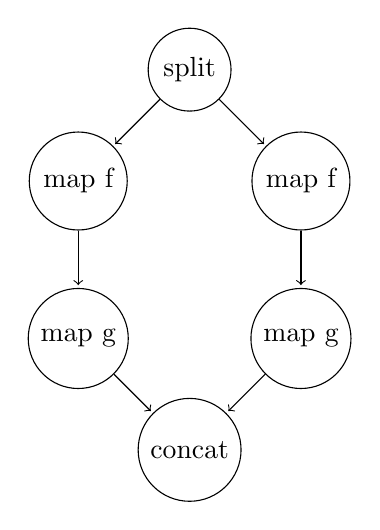
\begin{tikzpicture}[shorten >=1pt,node distance=2cm,on grid,auto] 
\node[state] (q_0) {split};
\node[state] (q_1) [below right = of q_0] {map f};
\node[state] (q_1_1) [below = of q_1] {map g};
\node[state] (q_2) [below left = of q_0] {map f};
\node[state] (q_2_1) [below = of q_2] {map g};
\node[state] (q_3) [below right =of q_2_1] {concat};
\path[->]
  (q_0) edge node {} (q_1)
  (q_0) edge node {} (q_2)
  (q_1) edge node {} (q_1_1)
  (q_2) edge node {} (q_2_1)
  (q_1_1) edge node {} (q_3)
  (q_2_1) edge node {} (q_3)
  ;
\end{tikzpicture}

\end{column}
\begin{column}[c]{5cm}
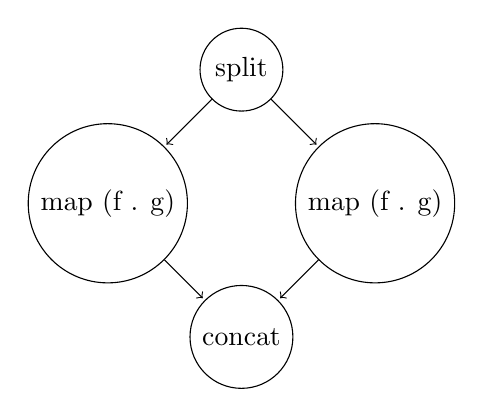
\begin{tikzpicture}[shorten >=1pt,node distance=2.4cm,on grid,auto] 
\node[state] (q_0) {split};
\node[state] (q_1) [below right = of q_0] {map (f . g)};
\node[state] (q_2) [below left = of q_0] {map (f . g)};
\node[state] (q_3) [below right =of q_2] {concat};
\path[->]
  (q_0) edge node {} (q_1)
  (q_0) edge node {} (q_2)
  (q_1) edge node {} (q_3)
  (q_2) edge node {} (q_3)
  ;
\end{tikzpicture}
\end{column}
\end{columns}
\end{frame}

\begin{frame}[fragile]
\frametitle{Array Fission}
Wrapper functions like {\tt fission-map} can either take
a plain array or two arrays that will eventually be concatenated.
\begin{lstlisting}
(define fission-map
  (lambda (f arr)
    (match arr
      [`(pull ,g ,len)
       (match-let ([`(,a ,b) (split arr)])
         `(concat ,(map f a) ,(map f b)))]
      [`(concat ,a ,b)
       `(concat ,(map f a) ,(map f b))])))
\end{lstlisting}
\end{frame}

\begin{frame}[fragile]
\frametitle{Array Fission}
{\tt fission-compute} takes either a pull array
or our {\tt concat} structure.
\begin{lstlisting}
(define fission-compute
  (lambda (arr)
    (match arr
      [`(pull ,f ,len)
       (compute arr)]
      [`(concat ,a ,b)
       (compute (concat a b))])))
\end{lstlisting}
We know how to efficiently concatenate arrays now, right?
\end{frame}

\begin{frame}[fragile]
\frametitle{Array Fission}
{\tt fission-fold} is similar, but it can also split the work 
of a fold on a pull array.
\begin{lstlisting}
(define fission-fold
  (lambda (f init arr)
    (match arr
      [`(pull ,g ,len)
       (match-let ([`(,a ,b) (split arr)])
         (f (fold f init a) (fold f init b)))]
      [`(concat ,a ,b)
       (f (fold f init a) (fold f init b))])))
\end{lstlisting}
\end{frame}

\begin{frame}
  \frametitle{Ongoing Work}
  We are still experimenting with fissioning in Accelerate. \\
  \hyperlink{http://dl.acm.org/citation.cfm?id=2808093}{See: {\em Converting Data-Parallelism to Task-Parallelism by Rewrites} in FHPC 2015.}
\end{frame}

\end{document}
